\chapter{Anisotropic Image-Driven Regularization}
\sectionmark{Anisotropic Image Driven Regularization}
The homogeneous regularizer of Horn and Schunck smoothes the flow field in all directions. This is a desirable property for internal pixels of an object, but not for pixels on the flow boundary. A homogeneous regularizer would smooth the flow field at pixels where one would expect the flow field to be discontinuous, which results in blurry flow edges. 
\section{Regularization according to image structure}
As one of the assumptions to the optical flow model is that different object has different brightness patterns, one would expect that flow boundaries coincide with image edges. Thus an amendment to this issue is to make a smoothness term which takes the gradients of the image into account, and smooths the flow field along image edges instead of across them. Such methods are called image-driven regularization methods. The anisotropic reguralizer of Nagel and Enkelmann \cite{Nagel:1986:ISC:11284.11285} performs smoothing along the image gradients and prevents smoothing across image edges. This is done by introducing a regularised projection matrix $P$, defined as
\begin{align*}
P(\nabla f) = \frac{1}{|\nabla f|^2 + 2 \kappa^2} (\nabla^{\bot} f (\nabla^{\bot})^T + \kappa^2 I),
\end{align*}
where $\nabla^{\bot} f= \left[-f_y, f_x \right]^T$, and $\kappa > 0$ is a regularization parameter. The smoothness term of Nagel and Enkelmann can now be written as the following
\begin{align*}
V_{AI}(\nabla u, \nabla v) = \nabla ^T u P(\nabla f) \nabla u + \nabla ^T v P(\nabla f) \nabla v,
\end{align*}
or written out 
\begin{align*}
V_{AI}(\nabla u, \nabla v) = \frac{\kappa^2}{|\nabla f|^2 + 2 \kappa^2} \left( u_{\textbf{s}_1}^2 + v_{\textbf{s}_1}^2 \right) + \frac{|\nabla f|^2 + \kappa^2}{|\nabla f|^2 + 2 \kappa^2} \left(u_{\textbf{s}_2}^2 + v_{\textbf{s}_2}^2 \right),
\end{align*}
where 
\begin{align}
\label{ID_smoothingDir}
&\textbf{s}_1 = \frac{1}{|\nabla f|}\begin{bmatrix}
f_x \\
f_y
\end{bmatrix},
& & \textbf{s}_2 = \frac{1}{|\nabla f|}\begin{bmatrix}
-f_y \\
f_x
\end{bmatrix}, & 
\end{align}
and $q_{\textbf{s}_i} = \textbf{s}_i^T \nabla u$ for $q = u, v$. That is, $q_{\textbf{s}_i}$ is the directional derivative of $q$ in the direction of the image gradient ($i=1$) or the orthogonal direction ($i=2$). This means that setting $\Theta=P$ in (\ref{EL_regu}) steers the diffusion so that flow vectors are smoothed along image edges and not across them.

\subsection{Discretizing the Nagel and Enkelmann smoothness term}
Setting $\Theta=P$ in (\ref{EL_regu}) leads to the following Euler-Lagrange system:
\begin{align*}
\frac{\partial M}{\partial u} - \frac{1}{\sigma^2} \text{div}(P \nabla u) = 0 \\
\frac{\partial M}{\partial v} - \frac{1}{\sigma^2} \text{div}(P \nabla v)= 0.
\end{align*}
Using the same discretizations for the derivatives as in \ref{sec: disc} one gets
\begin{align*}
(D^T D + \frac{1}{\sigma^2} L^TPL) \textbf{w} = - D^T \textbf{c}
\end{align*}
for the internal pixels and with Neumann boundary conditions given in equations (\ref{neumann1}) to (\ref{neumann8}). (Maybe some more details on discretization?)

\subsection{Results for the anisotropic image-driven regularization}
Experiments were run to find the best regularization parameter in the Nagel and Enkelmann smoothness term. The regularization parameter $\sigma$ found for the Horn and Schunck method is used to regularize the whole smoothness term. The resulting flow field for different choices of the regularization parameter $\kappa$, while keeping $\sigma$ constant, is shown in Figure (\ref{reguNE}). It is seen that choosing $\kappa = 0.8$ gives a fairly good segmentation of the object. Since the values for the gradient from the sobel derivative are relatively high, it is expected to also having to choose a relatively large value for $\kappa$ for sufficient regularization. Figure (\ref{reguNEHS}) compares the anisotropic smoothness term of Nagel and Enkelmann with $\kappa = 0.8$ with the homogeneous smoothness term of Horn and Schunck, both with using regularization parameter $\sigma = 0.003$. 

%\begin{figure}
%    \centering
%    \includegraphics[scale=0.8]{regularizationNE.eps}
%    \caption{Different choices for $\kappa$ using the Nagel and Enkelmann smoothness term}
%    \label{reguNE}
%\end{figure}
%
%\begin{figure}
%    \centering
%    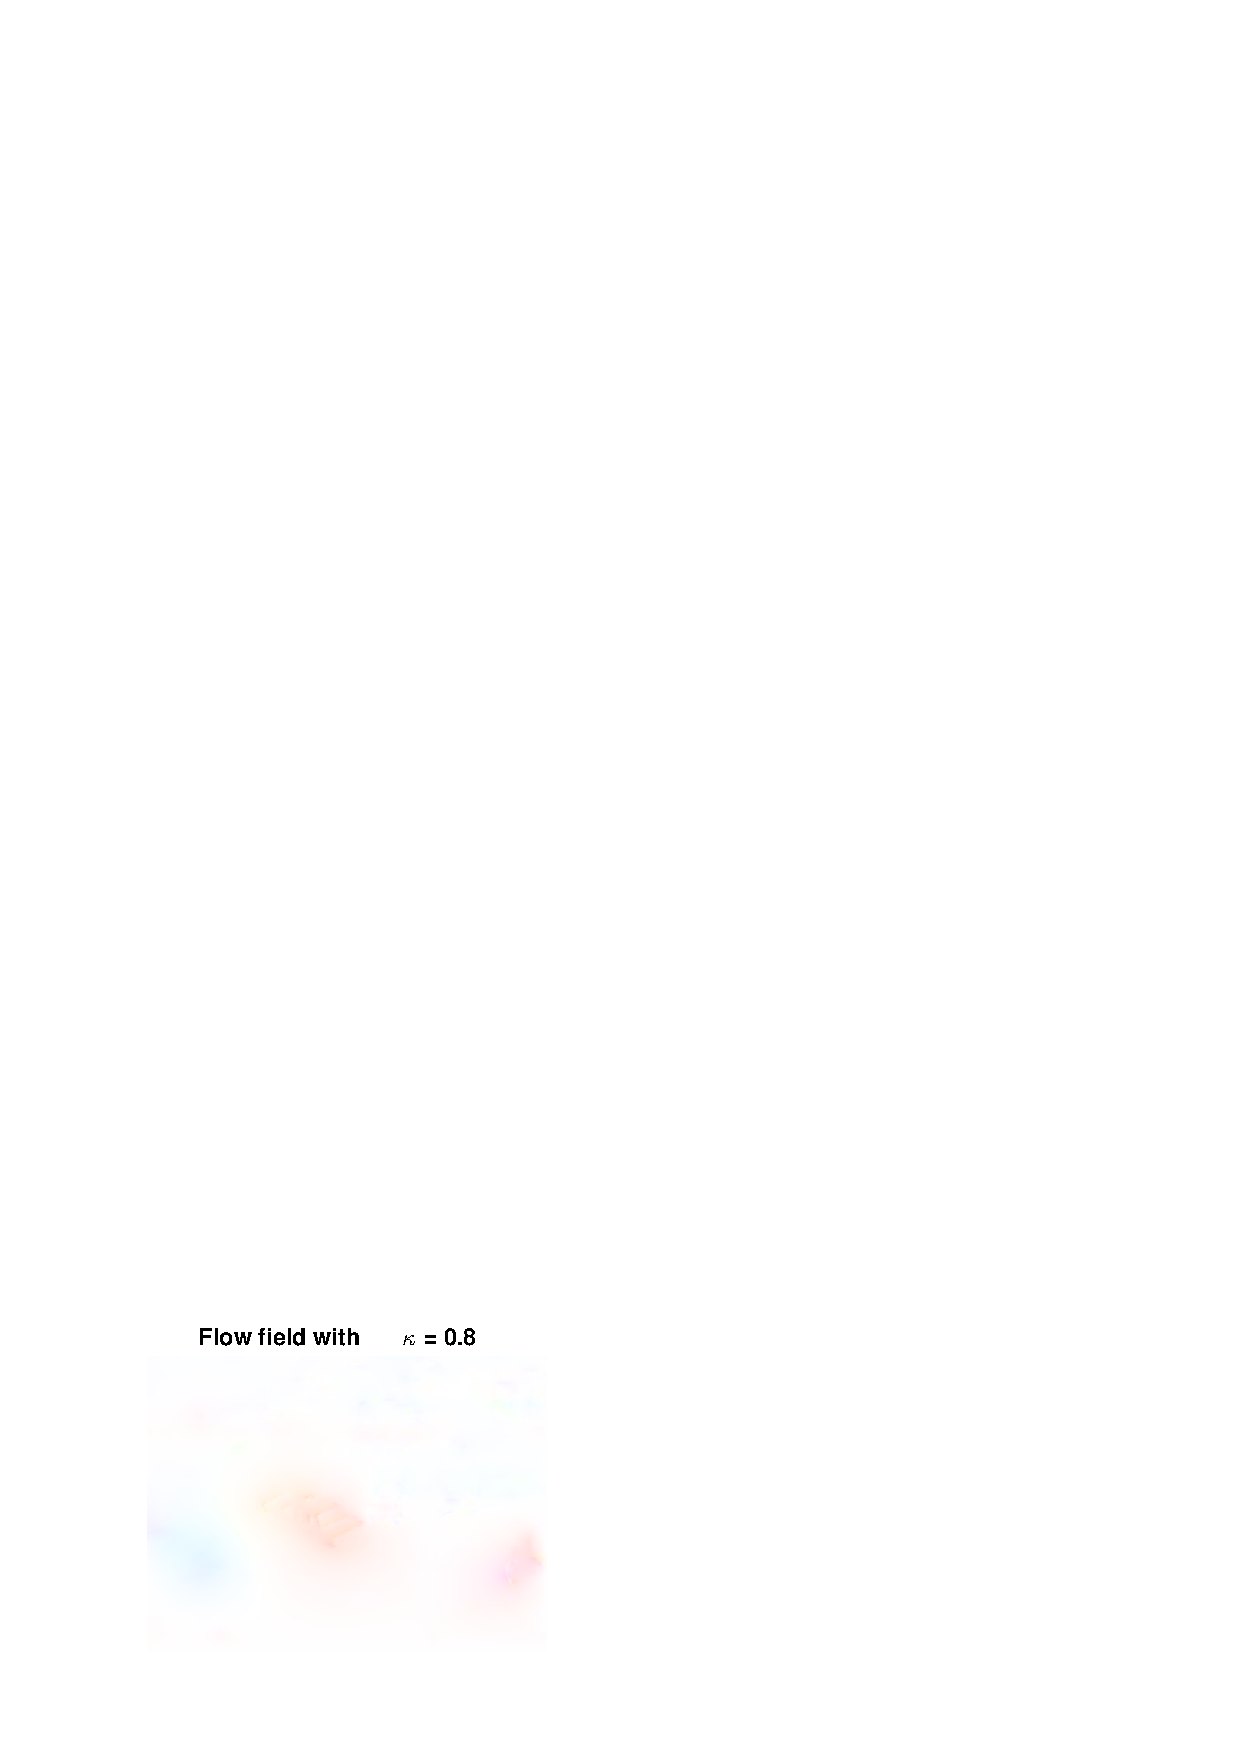
\includegraphics[scale=0.8]{NEregu}
%    \caption{Flow field with $\kappa= 0.8$ and $\sigma = 0.003$ using the Nagel and Enkelmann smoothness term.}
%    \label{reguNE_best}
%\end{figure}
%
%\begin{figure}
%    \centering
%    \includegraphics[scale=0.8]{reguNEHS.eps}
%    \subfloat[\label{NE_best} Anisotropic smoothness term.]{\hspace{.5\linewidth}}
%	\subfloat[\label{HS_best} Homogeneous smoothness term.]{\hspace{.5\linewidth}}
%	\caption{Comparison of the anisotropic and homogeneous smoothness term for given parameter choices.\label{humans}}
%    \label{reguNEHS}
%\end{figure}